\documentclass[aspectratio=169,10pt]{beamer}
\usetheme{Madrid}
\usecolortheme{seahorse}
\setbeamertemplate{navigation symbols}{}
\setbeamertemplate{footline}[frame number]

\usepackage[T1]{fontenc}
\usepackage[utf8]{inputenc}
\usepackage{tikz}
\usetikzlibrary{arrows.meta,positioning,fit,shapes.geometric}
\usepackage{booktabs}

\definecolor{HiderBlue}{HTML}{1565C0}
\definecolor{SeekerRed}{HTML}{C62828}
\definecolor{LLMTeal}{HTML}{00897B}
\definecolor{SoftBlue}{HTML}{EAF2FB}
\definecolor{SoftRed}{HTML}{FCEDEC}
\definecolor{SoftTeal}{HTML}{E7F5F2}
\tikzset{
  nodebox/.style={draw,rounded corners=2pt,align=center,inner sep=5pt,minimum height=8mm,font=\small},
  flow/.style={-{Stealth[length=2mm]},thick},
  hbox/.style={nodebox,draw=HiderBlue,fill=SoftBlue},
  sbox/.style={nodebox,draw=SeekerRed,fill=SoftRed},
  lbox/.style={nodebox,draw=LLMTeal,fill=SoftTeal},
  rolebox/.style={text width=2.1cm,minimum width=2.3cm}
}

\title{Graph-as-Policy for Hide-and-Seek}

\author{}
\institute{}
\date{November 5}

\begin{document}

\begin{frame}
  \titlepage
  \vspace{-6mm}

\end{frame}

\begin{frame}{Two methods, two different things get updated}
\small
\begin{columns}[T,onlytextwidth]
\column{0.49\textwidth}
\textbf{ADA: neural policy + PPO}
\begin{center}
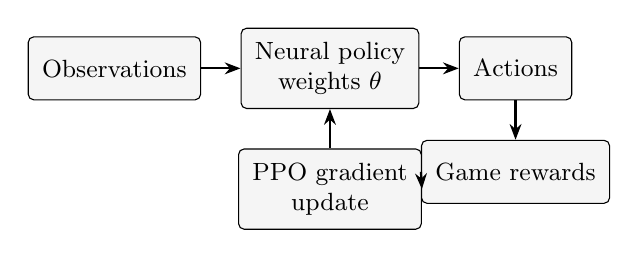
\begin{tikzpicture}[node distance=5mm]
  \node[nodebox,fill=gray!8] (obs) {Observations};
  \node[nodebox,fill=gray!8,right=of obs] (net) {Neural policy\\weights $\theta$};
  \node[nodebox,fill=gray!8,right=of net] (act) {Actions};
  \node[nodebox,fill=gray!8,below=of act] (rew) {Game rewards};
  \node[nodebox,fill=gray!8,below=of net] (ppo) {PPO gradient\\update};
  \draw[flow] (obs)--(net); \draw[flow] (net)--(act);
  \draw[flow] (act)--(rew);
  \draw[flow] (rew.west) -- (ppo.east);
  \draw[flow] (ppo.north) -- (net.south);
\end{tikzpicture}
\end{center}
Each rollout contributes reward/advantage data to a gradient update of the policy.
ADA also uses an opponent pool and adaptive task curriculum.

\column{0.49\textwidth}
\textbf{GaP: graph policies + proposal selection}
\begin{center}
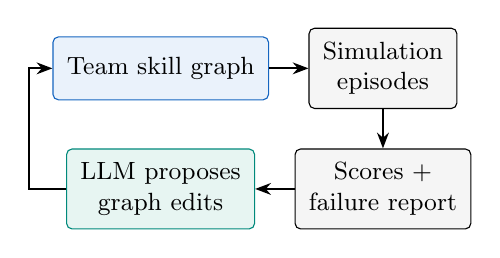
\begin{tikzpicture}[node distance=5mm]
  \node[hbox] (graph) {Team skill graph};
  \node[nodebox,fill=gray!8,right=of graph] (game) {Simulation\\episodes};
  \node[nodebox,fill=gray!8,below=of game] (report) {Scores +\\failure report};
  \node[lbox,left=of report] (llm) {LLM proposes\\graph edits};
  \draw[flow] (graph)--(game); \draw[flow] (game)--(report);
  \draw[flow] (report)--(llm);
  \draw[flow] (llm.west) -| ([xshift=-3mm]graph.west) |- (graph.west);
\end{tikzpicture}
\end{center}
Episodes evaluate graph proposals. They do \textbf{not} update neural weights.
\end{columns}
\vfill
\begin{alertblock}{Short version}
ADA learns weights with PPO. GaP searches over readable skill graphs using an LLM and simulator-based selection.
\end{alertblock}
\end{frame}

\begin{frame}{What is a graph policy? One graph per team}
\small
\begin{columns}[T,onlytextwidth]
\column{0.48\textwidth}
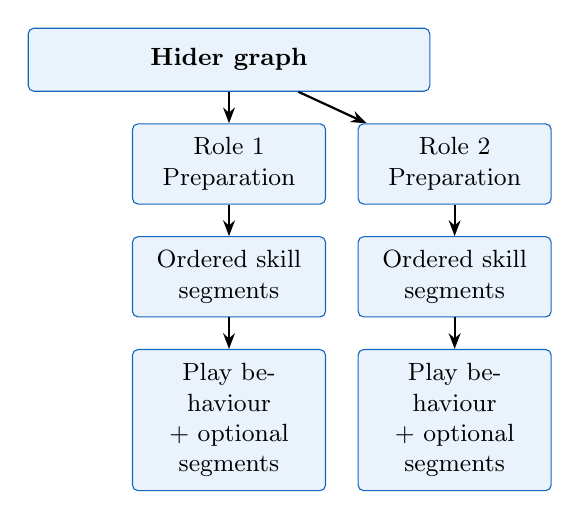
\begin{tikzpicture}[node distance=4mm]
  \node[hbox,minimum width=5.1cm] (ht) {\textbf{Hider graph}};
  \node[hbox,rolebox,below=of ht] (h0) {Role 1\\Preparation};
  \node[hbox,rolebox,right=of h0] (h1) {Role 2\\Preparation};
  \node[hbox,rolebox,below=of h0] (hp0) {Ordered skill\\segments};
  \node[hbox,rolebox,below=of h1] (hp1) {Ordered skill\\segments};
  \node[hbox,rolebox,below=of hp0] (hl0) {Play behaviour\\+ optional segments};
  \node[hbox,rolebox,below=of hp1] (hl1) {Play behaviour\\+ optional segments};
  \draw[flow] (ht)--(h0); \draw[flow] (ht)--(h1);
  \draw[flow] (h0)--(hp0); \draw[flow] (h1)--(hp1);
  \draw[flow] (hp0)--(hl0); \draw[flow] (hp1)--(hl1);
\end{tikzpicture}

\column{0.48\textwidth}
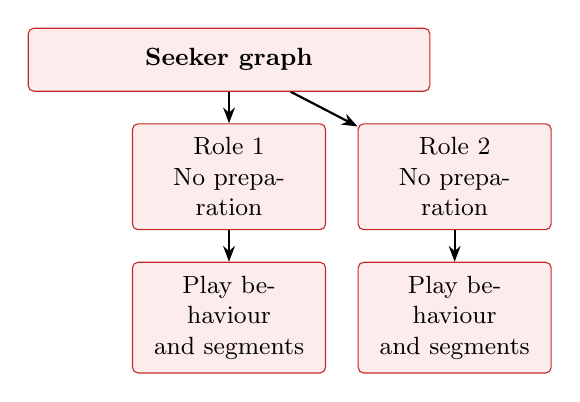
\begin{tikzpicture}[node distance=4mm]
  \node[sbox,minimum width=5.1cm] (st) {\textbf{Seeker graph}};
  \node[sbox,rolebox,below=of st] (s0) {Role 1\\No preparation};
  \node[sbox,rolebox,right=of s0] (s1) {Role 2\\No preparation};
  \node[sbox,rolebox,below=of s0] (sp0) {Play behaviour\\and segments};
  \node[sbox,rolebox,below=of s1] (sp1) {Play behaviour\\and segments};
  \draw[flow] (st)--(s0); \draw[flow] (st)--(s1);
  \draw[flow] (s0)--(sp0); \draw[flow] (s1)--(sp1);
\end{tikzpicture}
\end{columns}

\vspace{2mm}
\begin{block}{Graph vocabulary}
Each role contains a play behaviour (e.g. \texttt{search}, \texttt{chase}) and ordered segments. A segment composes primitive skills: acquire an object, deliver it to a target, optionally lock/release.
\end{block}
\end{frame}

\begin{frame}{One GaP round: propose, rehearse, select}
\centering
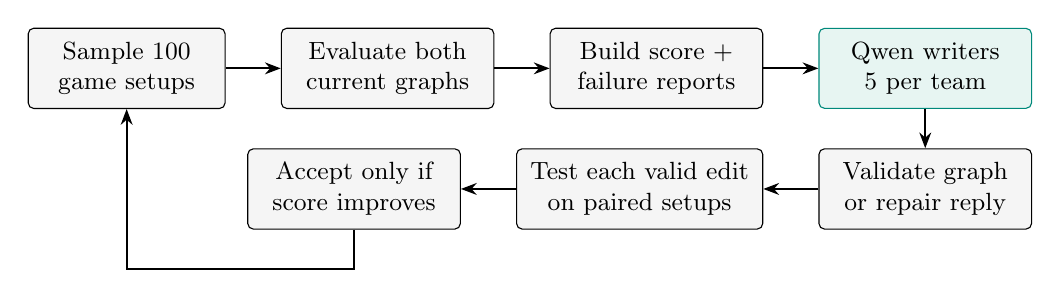
\begin{tikzpicture}[node distance=5mm and 7mm]
  \node[nodebox,fill=gray!8,minimum width=2.5cm] (sample) {Sample 100\\game setups};
  \node[nodebox,fill=gray!8,right=of sample,minimum width=2.7cm] (base) {Evaluate both\\current graphs};
  \node[nodebox,fill=gray!8,right=of base,minimum width=2.7cm] (feedback) {Build score +\\failure reports};
  \node[lbox,right=of feedback,minimum width=2.7cm] (llm) {Qwen writers\\5 per team};
  \node[nodebox,fill=gray!8,below=of llm,minimum width=2.7cm] (valid) {Validate graph\\or repair reply};
  \node[nodebox,fill=gray!8,left=of valid,minimum width=2.7cm] (test) {Test each valid edit\\on paired setups};
  \node[nodebox,fill=gray!8,left=of test,minimum width=2.7cm] (select) {Accept only if\\score improves};
  \draw[flow] (sample)--(base); \draw[flow] (base)--(feedback); \draw[flow] (feedback)--(llm);
  \draw[flow] (llm)--(valid); \draw[flow] (valid)--(test); \draw[flow] (test)--(select);
  \draw[flow] (select.south) -- ++(0,-5mm) -| (sample.south);
\end{tikzpicture}

\vspace{3mm}
\begin{columns}[T,onlytextwidth]
\column{0.53\textwidth}
\footnotesize
\textbf{Current settings:}
\begin{itemize}\setlength{\itemsep}{1pt}
  \item 5 continuous LLM writers per team; collect proposals for 45 seconds. The number received varies.
  \item 100 paired game episodes per current graph and per unique, valid proposal.
  \item Both teams update each round. Total episodes vary with valid, non-duplicate proposals; acceptance requires a score gain of 0.05 after a small complexity penalty.
\end{itemize}
\column{0.43\textwidth}
\begin{alertblock}{What “learning” means here}
The graph stays fixed during each episode. Between episodes, the LLM proposes edits and the simulator judges them.
\end{alertblock}
\end{columns}
\vfill

\end{frame}

\end{document}